\section{Circulation conservative du champ électrostatique. Potentiel électrostatique}

    \subsection{Circulation entre deux points du champ créé par une charge ponctuelle}

        On considère le système décrit par la Figure~\ref{fig:circulation_deux_points_champ_cree_charge_ponctuelle}.

        \begin{figure}
            \centering
            \tikzsetnextfilename{circulation_deux_points_champ_cree_charge_ponctuelle}
            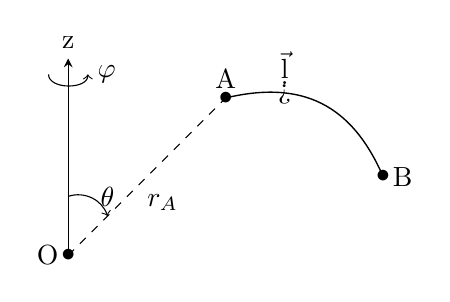
\begin{tikzpicture}[scale=1]  
                % \helpgrid{3}{3}
                \coordinate (O) at (0,0);
                \node at (O) {$\bullet$};
                \node at (O) [left] {O};
                \coordinate (A) at (2,2);
                \coordinate (B) at (4,1);
                \node at (B) {$\bullet$};
                \node at (B) [right] {B};
                \draw [line width=0.5pt] (A) edge[bend left=40,distance=1cm] (B);
                \node at (2.75,2.05) {>};
                \node at (2.75,2.05) [above]{$\vec{\d l}$};
                \draw [->, -stealth] (O)--(0,2.5) node [above] {z};
                \draw[dashed] (O)--(A) node [below, midway, shift={(0.2,-0.1)}] {$r_{A}$};
                \node at (A) {$\bullet$};
                \node at (A) [above] {A};
                \draw [->] (0,0.75) to [bend left=45] (0.5,0.5) node [above] {$\theta$};
                \draw [->] (-0.25,2.3) to [bend right=90] (0.25,2.3) node [right] {$\varphi$};
            \end{tikzpicture}
            \caption{Circulation entre deux points du champ créé par une charge ponctuelle.}    
            \label{fig:circulation_deux_points_champ_cree_charge_ponctuelle}
        \end{figure}
        
        On cherche la circulation de $\vec{E}$ entre A et B, c'est-à-dire 
        \begin{equation}
            \int_{A}^{B}\vec{E}\cdot\vec{\d l}.
        \end{equation}

        En coordonnées sphériques, on a
        \begin{equation}
            \vec{\d l}=\d r\vec{u_r}+r\d\theta\vec{u_{\theta}}+r\sin\theta\d\varphi\vec{u_{\varphi}}.
        \end{equation}

        Ainsi,
        \begin{equation}
            \int_{A}^{B}\vec{E}\cdot\vec{\d l}=\frac{Q}{4\pi\varepsilon_{0}}\left(\frac{1}{r_{A}}-\frac{1}{r_{B}}\right),
        \end{equation}
        qui ne dépend que de $A$ et $B$ et pas du chemin choisi. Par définition, le potentiel électrostatique $V(M)=V(x,y,z)=V(r,\theta,\varphi)$ est défini par 
        \begin{equation}
            \int_{A}^{B}\vec{E}\cdot\vec{\d l}=V(A)-V(B),
        \end{equation}
        et on a $[V]=\si{\volt}$.

    \subsection{Potentiel créé par une charge ponctuelle}

        On a 
        \begin{equation}
            \boxed{
                V(M)=V(r)=\frac{Q}{4\pi\varepsilon_{0}r},
            }
        \end{equation}
        où l'on prend la constante nulle à l'infini. Pour une collection de charges ponctuelles, on utilise le principe de superposition :
        \begin{equation}
            \boxed{
                V(M)=\frac{1}{4\pi\varepsilon_{0}}\sum_{i=1}^{N}\frac{Q_i}{r_i}.
            }
        \end{equation}

    \subsection{Circulation du champ électrostatique le long d'un contour fermé orienté}

        Pour deux points $A$ et $B$ du contour $\mathcal{C}$, si $\vec{\d l_{1}}$ connecte $A$ à $B$ et $\vec{\d l_{2}}$ connecte $B$ à $A$, alors 
        \begin{equation}
            \oint_{\mathcal{C}}\vec{E}\cdot\vec{\d l}=\int_{A}^{B}\vec{E}\cdot\vec{\d l_{1}}+\int_{B}^{A}\vec{E}\cdot\vec{\d l_{2}}=V(A)-V(B)+V(B)-V(A)=0,
        \end{equation}
        donc $\vec{E}$ est à circulation conservative. C'est une équation intégrale.

    \subsection{Lien local entre le champ électrostatique et le potentiel électrostatique. Opérateur gradient}

        Pour deux points $M(x,y,z)$ et $M'(x+\d x,y+\d y,z+\d z)$ connectés par $\vec{\d l}=(\d x,\d y, \d z)$, on a
        \begin{align}
            \vec{E}\cdot\vec{\d l}
            &=
            \vec{E}\cdot\vec{MM'},\\
            &=
            V(M)-V(M'),\\
            &=
            E_x\d x+E_y\d y+E_z\d z,\\
            &=
            V(x,y,z)-V(x+\d x,y+\d y,z+\d z),\\
            &=\d x\frac{\partial V}{\partial x}(x,y,z)+\d y\frac{\partial V}{\partial y}(x,y,z)+\d z\frac{\partial V}{\partial z}(x,y,z),
        \end{align}
        ceci étant valide pour tout déplacement $\vec{\d l}$, donc 
        \begin{equation}
            E_x\d x+E_y\d y+E_z\d z=-\d V=-\frac{\partial V}{\partial x}\d x-\frac{\partial V}{\partial y}\d y-\frac{\partial V}{\partial z}\d z.
        \end{equation}

        Ainsi, 
        \begin{equation}
            \boxed{
                \vec{E}=-\begin{pmatrix}
                    \frac{\partial V}{\partial x}\\
                    \frac{\partial V}{\partial y}\\
                    \frac{\partial V}{\partial z}
                \end{pmatrix}
                =-\vec{\grad}V.
            }
        \end{equation}

        En coordonnées cartésiennes, on a simplement $\vec{E}=-\vec{\nabla}V$. C'est une équation locale.

    \subsection{Énergie potentielle d'une charge ponctuelle dans un champ extérieur : sens physique du potentiel électrostatique}

        On reprend le système décrit par la Figure~\ref{fig:circulation_deux_points_champ_cree_charge_ponctuelle}. On souhaite calculer cette fois-ci le travail développé par la force électrostatique. On a 
        \begin{align}
            W_{A\to B}^{\text{el}}
            &=
            \int_{A}^{B} \vec{F}_{\text{el}}\cdot\vec{\d l},\\
            &=
            \int_{A}^{B}q\vec{E}^{\text{ext}}\cdot\vec{\d l},\\
            &=
            -q\int_{A}^{B}\d V^{\text{ext}},\\
            &=
            -q\left[
                V^{\text{ext}}(B)-V^{\text{ext}}(A)
            \right].
        \end{align}

        Ainsi, il existe une énergie potentielle $E_{p}^{\text{ext}}$ telle que 
        \begin{equation}
            W_{A\to B}^{\text{el}}=-\Delta E_{p}^{\text{ext}},
        \end{equation}
        d'où $E_{p}^{\text{ext}}=qV^{\text{ext}}$. Par convention, on prend $E_p^{\text{ext}}(\infty)=0$.

        On définit aussi l'électron-volt. Il 'agit de l'énergié à fournir pour amener un électron du potentiel 0\si{\volt} au potentiel 1\si{\volt}. Ainsi, 
        \begin{equation}
            \boxed{
                1\si{\electronvolt}=e\times1\si{\volt}=1,6.10^{-19}\si{\joule}.
            }
        \end{equation}        